
%
% foundations - vis
%

\section{Visualization}
\label{chapter:foundations-vis}

In the following chapter, foundations for visualizing clusters on a map will be discussed. Basics of geographic visualization and their driving forces lead to abstraction and clustering as a tool for simplifying information that needs to be communicated. Visual variables as well as classification approaches for geovisualization will be reviewed in order to review existing concepts for displaying aggregated data on a map.

Visualization is driven by the basic belief that `seeing' is a good way of understanding and generating knowledge. Humans have a very well developed sense of sight, which is underlined by the fact, that more of 50 percent of the neurons in our brain are used in vision.~\cite{vislecture}. 

MacEachren \& Kraak~\cite{maceachren-geovis} define, that ``Geovisualization integrates approaches from visualization in scientific computing (ViSC), cartography, image analysis, information visualization, exploratory data analysis (EDA), and geographic information systems (GISystems) to provide theory, methods, and tools for visual exploration, analysis, synthesis, and presentation of geospatial data (any data having geospatial referencing).'' In his lecture notes on ``Geographic visualization'', Martin N\"{o}llenburg adds that more human-centered definitions exist and observes that the user's needs have to be taken into account for effective geovisualization techniques~\cite{noellenburg11geovis}.


The \textbf{goals of geovisualization} can be summarized using the \textit{map use cube} by MacEachren and Kraak \cite{MacEachren07cartovis}, which is illustrated in figure \ref{fig:geovis-cube}. The goals \textit{exploration, analysis, synthesis and presentation} are classified amongst three dimensions:

\begin{itemize}

\item The type of \textit{task} varies from \textit{knowledge construction} to \textit{information sharing}. While the first is about revealing unknowns and constructing new knowledge, the latter will primarily share existing knowledge.

\item The amount of \textit{interaction} ranges from high to low. A low level of interaction means a rather passive consumption of knowledge, instead a high level will allow the user to actively influence the visualization.

\item The \textit{users} of visualization are classified between public and private audiences. A single, private user might require different visualization techniques than large, public audiences.

\end{itemize}

In the given model of the map use cube, the goals of exploring,analyzing, synthesizing and presenting shift between the extremes of the three defined aspects. The first goal of exploring is classified as a task of knowledge construction, based on high interaction and targeted at a rather private audience. On the other hand, presenting is a task of information sharing that requires a low amount of interaction but is suitable for public audiences~\cite{noellenburg11geovis}.  

\begin{figure}[h]
  \begin{center}
    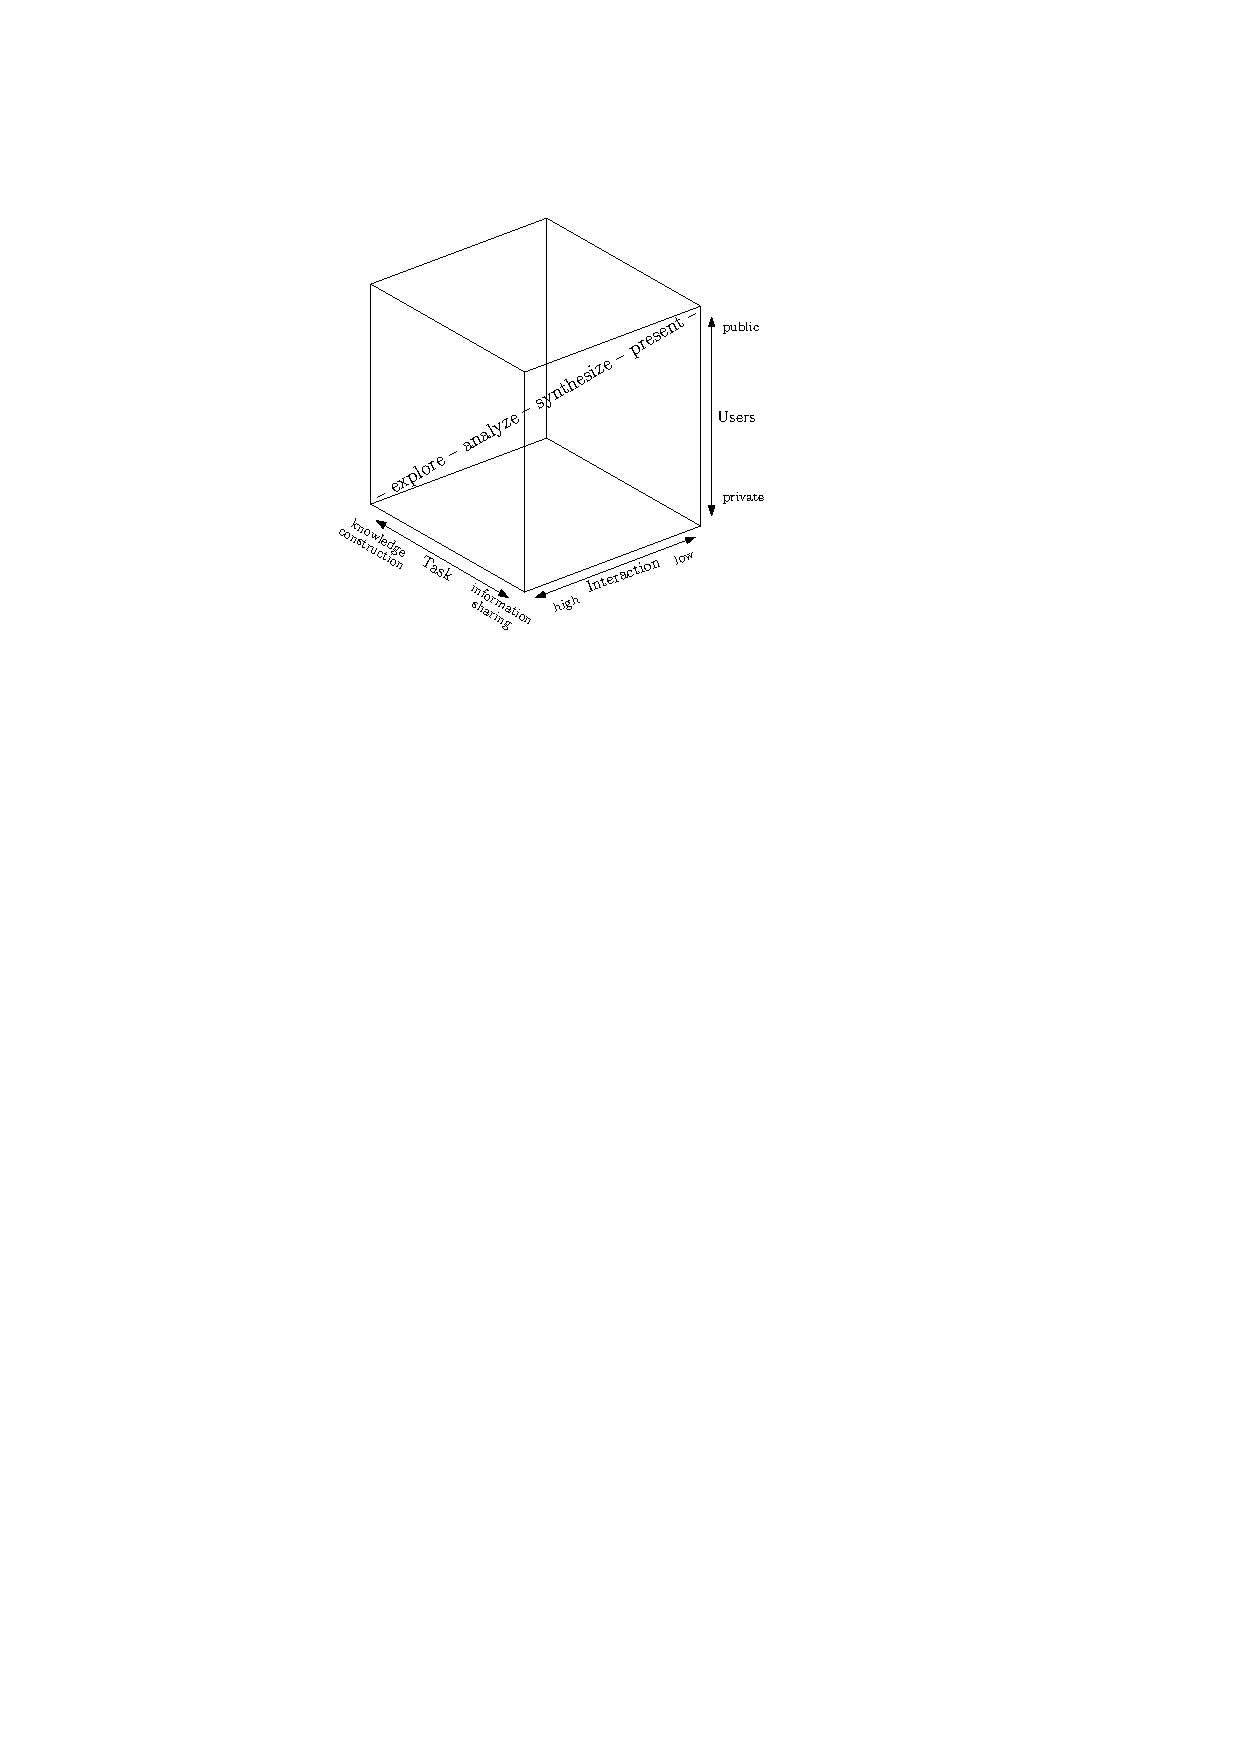
\includegraphics[width=0.65\textwidth]{figures/geovis_goals.pdf}
    \caption{The map use cube after MacEachren and Kraak \cite{MacEachren07cartovis} characterizing geovisualization goals in a three-dimensional space by their level of interaction, their audience, and the addressed tasks.~\cite{noellenburg11geovis}.}
    \label{fig:geovis-cube}
  \end{center}
\end{figure}


Cognitive aspects of visualization help us understand, how visual thinking works. Complex input is abstracted on the retina of the human eye in order to match these abstractions against a vast collection of patterns from experience. Despite generating realistic images, visualization can help generate new ideas by using abstraction to communicate patterns. The idea is to allow the user to join insight, draw conclusions and interact with the data by presenting it in a visual form that reduces the cognitive work needed to perform the given task~\cite{MACEACHREN90apattern, keim2001vis, noellenburg11geovis}. 

Various scientific publications~\cite{phillips82clutter, MACEACHREN90apattern, keim2001vis, harvey2008primer, ellis08clutter, Delort10vis, noellenburg11geovis} that have been researched for this thesis mention the importance of using abstraction for efficiently visualizing information. Especially maps can only highlight interesting information by filtering out unnecessary details of the environment. For example, a road map is better visualized on a clear background instead of satellite images that would distract the user from the primary goal of finding directions. The challenge is to balance realism and abstraction in geovisualization depending on the problem~\cite{noellenburg11geovis}.

\subsection{Visual variables}
\label{chapter:vis-variables}

\begin{figure}[h]
  \begin{center}
    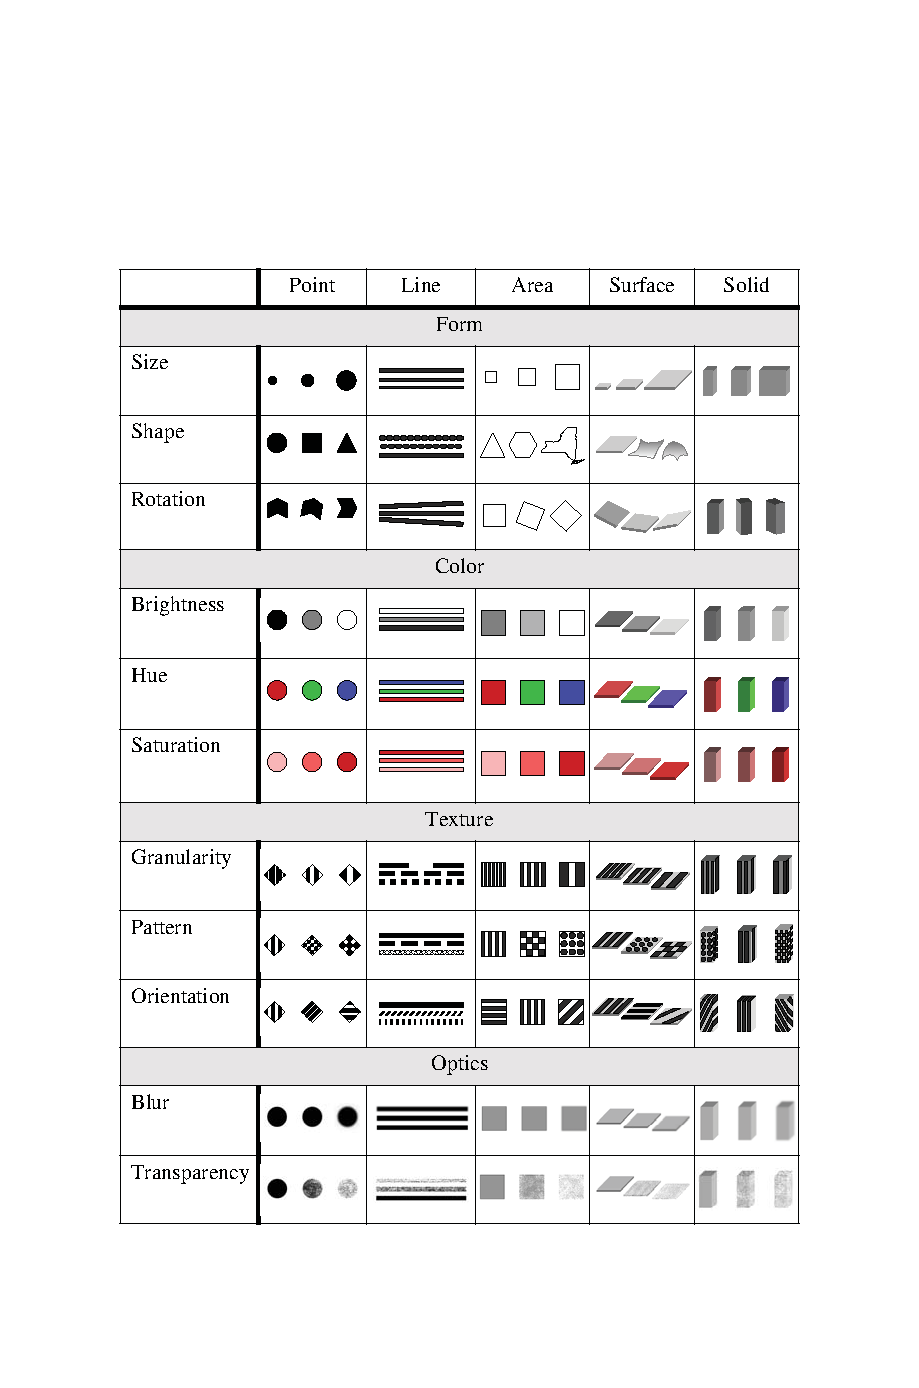
\includegraphics[width=0.8\textwidth]{figures/aesthetic_attributes.pdf}
    \caption{Aesthetic Attributes by Geometry~\cite{Wilkinson05grammar}.}
    \label{fig:aesthetic-attributes}
  \end{center}
\end{figure}

Information on a map is represented by symbols, point, lines or areas with properties such as color and shape. Bertin~\cite{bertin67graphics, bertin83graphics} has described the fundamental graphic variables for map and graphic design. While being written for hand-drawn maps on paper, the concepts described by Bertin are still applied in todays digital mapping applications and have been further developed by MacEachren~\cite{MacEachren95maps}.

The main variables, introduced by Bertin are: location, size, value, texture, color, orientation and shape. MacEachren adds crispness, resolution, transparency and arrangement to the list and splits up color into its value of brightness, saturation and hue. Figure \ref{fig:aesthetic-attributes} describes a similar list of aesthetic attributes by different geometries and groups the variables regarding form, color, texture and optics.

Each variable has a different potential for visualizing data of categorical information (nominal and ordinal) or numerical information (including intervals and ratios). For example, the size of a point can be used to describe a numeric ratio and different shapes may be used to distinguish items based on categories. On the other hand, different texture patterns only offer a limited set of possibilities and size shouldn't be used for describing nominal properties~\cite{noellenburg11geovis, MacEachren95maps}. 

\subsection{Visual data exploration techniques}
\label{vis-data-techniques}

Depending on the task and the type of data to be shown, different forms of visualization and techniques for exploring the data exist. Daniel A. Keim~\cite{keim2001vis} classifies such techniques using three criteria as depicted in figure \ref{fig:visual-techniques}: the data type to be visualized, the technique itself and the interaction and distortion method~\cite{Delort10vis}:

\begin{itemize}

\item The \textbf{data type} may be one-dimensional (as for example temporal data), two-dimensional (geographical maps), multi-dimensional (relational tables), text and hypertext (articles and web documents), hierarchies and graphs (networks) and algorithms and software (such as debugging operations).

\item The \textbf{visualization techniques} are classified into standard 2d/3d displays (x-y plots and landscapes), geometrically-transformed displays (parallel coordinates), iconic displays (glyphs), dense pixel displays (recursive pattern) and stacked displays (tree maps).

\item Finally, the third dimension describes the \textbf{interaction technique} being used, such as dynamic projection, interactive filtering, zooming, distortion and link \& brush approaches.

\end{itemize}

\begin{figure}[h]
  \begin{center}
    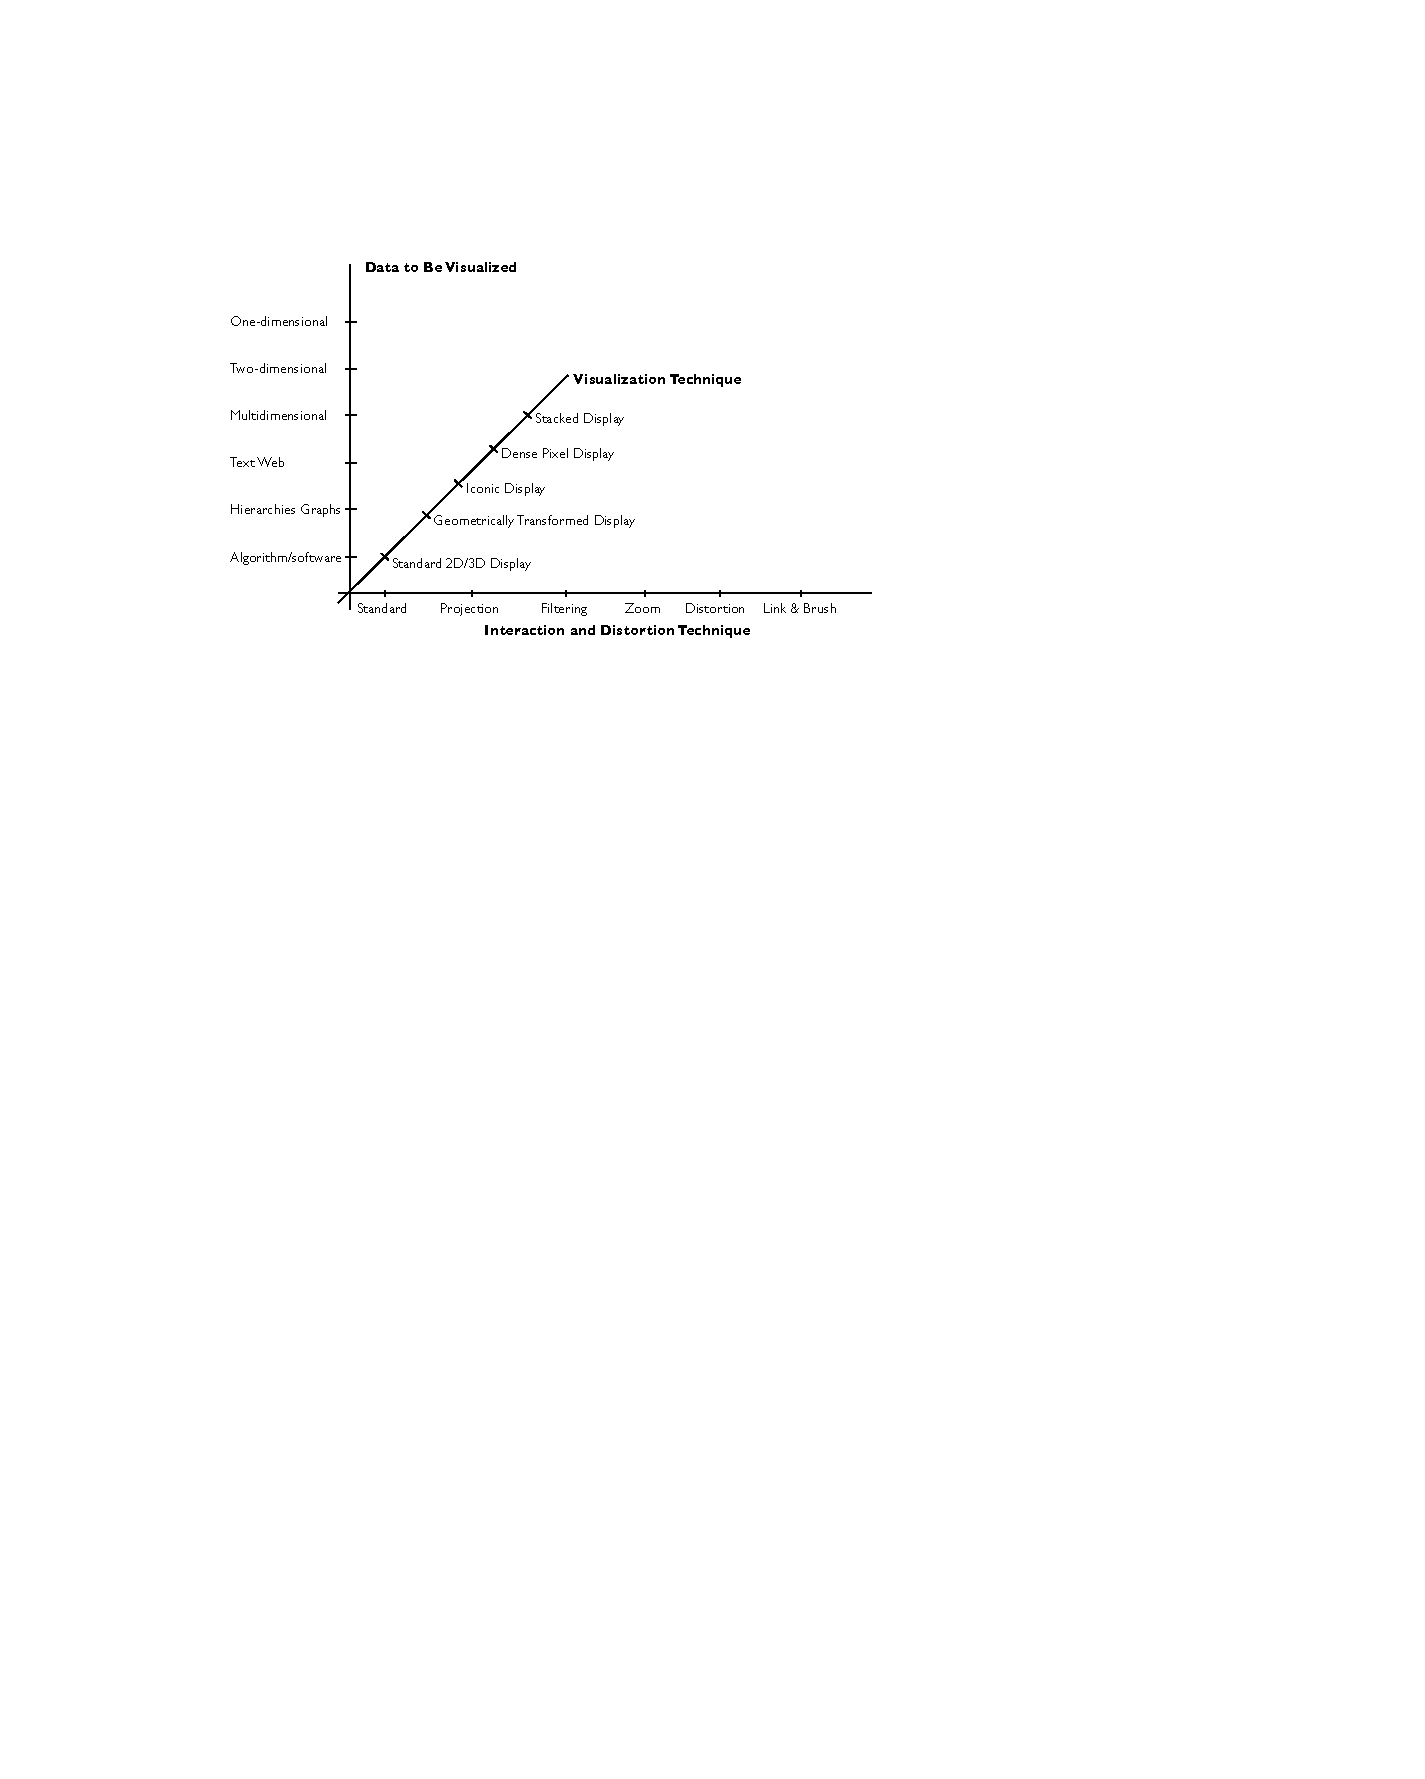
\includegraphics[width=1\textwidth]{figures/classes_visual_techniques.pdf}
    \caption{Classification of visual data exploration techniques based on~\cite{keim2001vis}.}
    \label{fig:visual-techniques}
  \end{center}
\end{figure}


With regard to visualizing clusters on a map, the visualization technique may be considered from two different view points:

\begin{itemize}

\item the visualization of the \textit{entire map} with clustered points on it, as well as

\item the visualization of an \textit{individual cluster}, placed on the map.

\end{itemize}

A typical map for representing spatially clustered data is based on a least two-dimensional data, containing latitude and longitude information of cluster items. The map is presented in planar space, which classifies it amongst standard 2d/3d displays. Common interaction techniques for maps are zooming and panning which allow to explore the 2-dimensional space and reveal details.

The visualization of individual clusters on the map is likely to be classified amongst iconic displays. During the clustering process, individual points get aggregated, which potentially leads to multivariate aggregate information of item properties. Depending on the level of detail that clusters should expose, more complex visualization techniques may be possible. 

Approaches for visualization techniques of the entire map and individual clusters will be discussed further in chapter TODOREF.

\subsection{Clutter reduction}
\label{clutter-reduction}

Clutter reduction is a way to enhance readability and general performance of maps. An early publication about \textit{visual clutter} on maps by Richard J. Phillips and Liza Noyes~\cite{phillips82clutter} states that ``reducing visual clutter improves map reading performance''. This especially becomes true for visualizing large data sets on maps, so that properties of the data items are hardly visible. Clutter reduces the background visibility and prevents the user from understanding structure and content of the data being presented~\cite{harvey2008primer, Delort10vis}.

Clustering of course is the approach for clutter reduction that is primarily being investigated for this thesis. In order to review the effectiveness and limitations of clustering, as well as the relationship that it has to other techniques in that field, it is helpful to review the ``Clutter Reduction Taxonomy'' by Geoffrey Ellis and Alan Dix~\cite{ellis08clutter}. It distinguishes between three main types of clutter reduction techniques:

\begin{itemize}

\item \textbf{appearance}: alter the look of data items by using techniques like \textit{sampling}, \textit{filtering}, \textit{changing point sizes}, \textit{changing opacity} or \textit{clustering}.

\item \textbf{spatial distortion}: displace the data items in ways as \textit{point/line displacement}, \textit{topological distortion}, \textit{space-filling}, \textit{pixel-plotting} or \textit{dimensional reordering}.

\item \textbf{temporal}: use animation to reveal additional information.

\end{itemize}

In a next step, the stated techniques have been evaluated against a list of 8 high-level criteria. For this thesis, the relevant information for the clustering technique will be outlined for each criterium:

\begin{enumerate}

\item \textit{avoids overlap}
\\ The major benefit is to reduce clutter, provide the ability of seeing and identifying patterns, have less hidden data as well as giving more display space to points. Clustering can be used in such a way tol avoid over plotting by representing groups of points as single points.

\item \textit{keeps spatial information}
\\ If a clutter reduction technique maintains the correct coordinates of items is relevant, but the study also states that maintaining relative positions might have greater influence on orientation than just the exact coordinates. Clustering looses the spatial information of individual points, but using aggregate values like the centroid a cluster as the position can be used for compensation. 

\item \textit{can be localized}
\\ The term localization is used to specify, if the display can be reduced to a specific region. This is usually provided by focus and context techniques that reveal information underneath by zooming into an area. The study doesn't make a clear decision regarding the applicability of localization for clustering and states that different properties for spatial and non-spatial clustering apply. In the case of spatial clustering, localization is definitely possible and has been implemented, see chapter \ref{chapter:realization}.  

\item \textit{is scalable}
\\ Scalability of the clutter reduction technique with regards to large amounts of data is the goal of this criterium. The study admits that the meaning of large datasets is vaguely quantified. As one of the main goals for this thesis is to enhance performance for large data set by using clustering, the technique is expected to satisfy this condition. Of course the range of scalability depends on the implemented clustering algorithm. Also refer to the time complexity definitions in chapter \ref{clustering-algorithms}. 

\item \textit{is adjustable}
\\ If the user is able to control aspects of the visual display and adjust parameters of the system that influence the degree of display clutter. Scientific methods in cluster analysis tend to offer a a higher level of interactivity while public facing clustering application limit the amount of interactivity to controlling cluster sizes and the previously discussed localizing feature. 

\item \textit{can show point/line attribute}
\\ The goal is to map attributes of the data to properties like color, shape or opacity of the displayed points or lines. For clustering, this feature can be used in order to display aggregates of the multivariate data results from the clustering process. Further information can be found in chapter TODOREF.

\item \textit{can discriminate points/lines}
\\ Being to able to identify individual data items within a crowded display is the goal of this criterium. The study states the capability of clustering for detecting outliers as well as creating groups of points in order to satisfy this criterion. On the other hand, this classification appear unclear, as the grouping process of clustering hides individual information by definition and only makes it accessible by request or localization. 

\item \textit{can see overlap density}
\\ This helps to gauge the amount of overplotting, see where higher density regions are and understand the distribution of data underlying the visualization. Clustering can show the amount of items within clusters by using visual indicators as point size, opacity and color.  

\end{enumerate}

TODO OUTRO
